Systematic uncertainties treatment for \ZZ\ analysis is similar to the
\WW\ one. This section describes only systematic effects that are
different from \WW{}.

\subsection{\ZZ\ and \WZ\ background}

The $\wz$ and $\zz$ backgrounds are the ireducible backgrounds to the 
Higgs $\to$ \ZZ\  search. We do not have a data-driven estimate yet, 
the shapes are taken from MC. 
Similar to the \WW{} background treatment as in the $\hww$ analysis, 
we accounts for the effects of therorectical uncertainties due to the 
missing higher order calculations. 

For the $\zz$ background, the central shape is simulated with 
Madgraph generator with the event-by-event reweighting in the 
$\Z$ boson $p_T$ spectrum to match the NLO calculation by MCFM.
We assess the effects of QCD scales by comparing the central shape 
with an alternative generator available in CMS, which is Pythia. 
As an alternative approach, we can also assess the QCD scale variations of $\ZZ$ background by 
compute the event-by-event k-factor with the normalization and 
factorization scales independently. Figure~\ref{fig:zzsyst_hzz} show the 
shape variations of \ZZ\  background estimated for the $m_H=250\GeVcc$ selection. 

Similarly, the central shape of $\wz$ background is simulated with 
Madgraph. We compare the shapes to the ones generated with Pythia to 
assess the theoretical uncertainties. 
On the other hand, the $\WZ$ shapes can be further validated with data in 
a control region of events with 3 leptons with increasing luminosity. 
Figure~\ref{fig:wzsyst_hzz} show the shape variations of \WZ\ 
background estimated for the $m_H=250\GeVcc$ selection. 

%%%%%%%%%%%%%%%%%%%%%%%%
\begin{figure}[!htbp]
\begin{center}
\subfigure[]{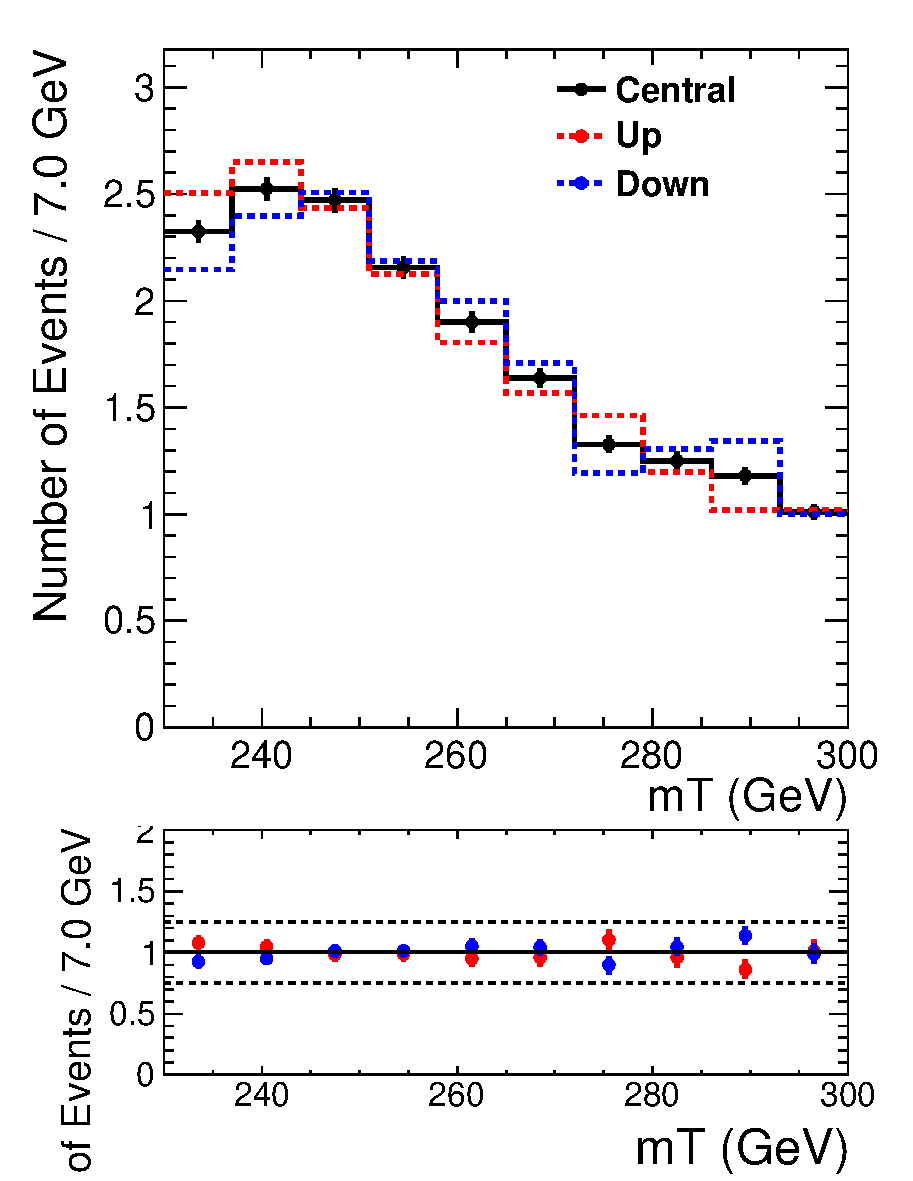
\includegraphics[width=0.49\textwidth]{figures/ZZ_ZZBounding_mT_mH250_ee_lin.pdf}}
\subfigure[]{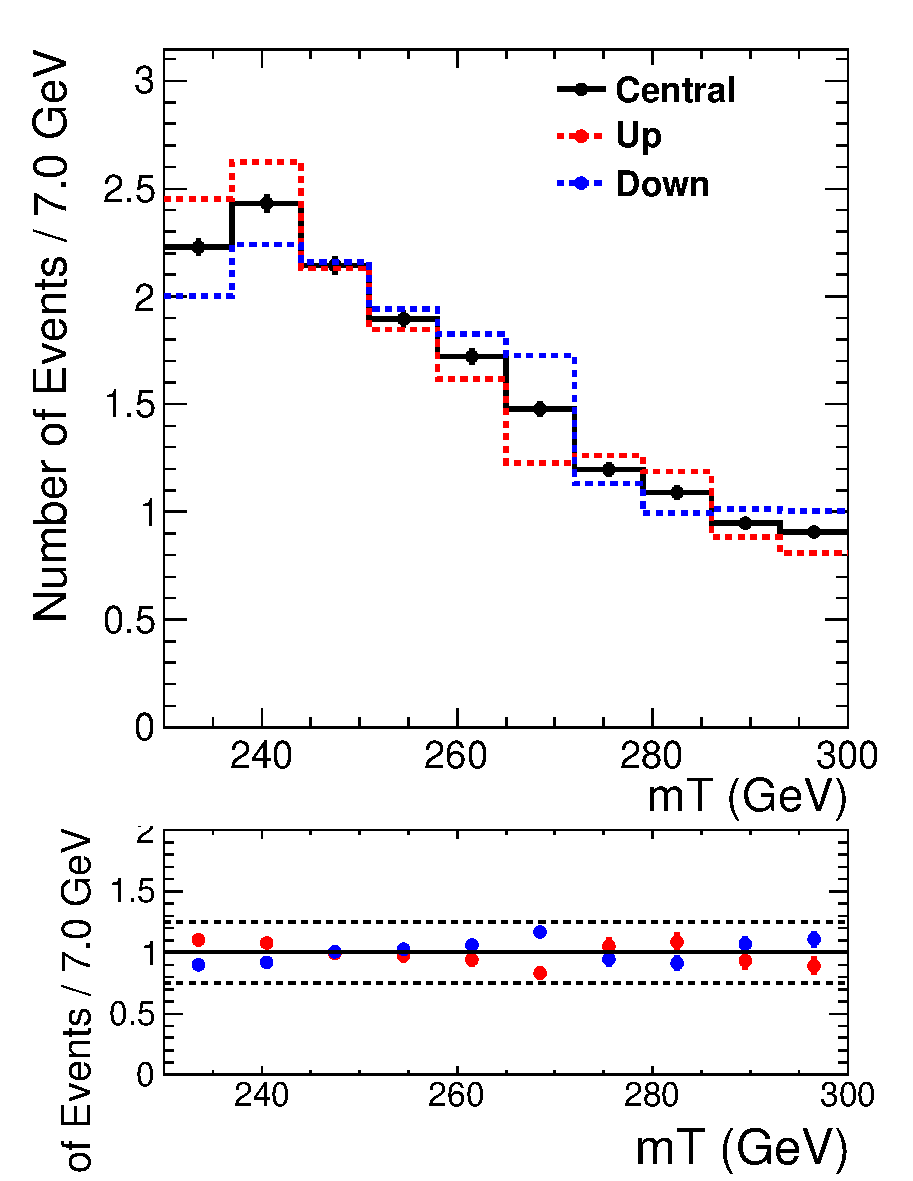
\includegraphics[width=0.49\textwidth]{figures/ZZ_ZZBounding_mT_mH250_mm_lin.pdf}}\\
\caption{$m_T$ distribution for $\ZZ$ for the ee (left) and $\mu\mu$ (right) final states. 
The central shape is taken from Madgraph with $p_T$ spectrum reweighted to match 
the NLO calcuation. The up histogram is taken from Pythia with the down 
histogram taken as a variation mirroring the difference between up and central. 
}
\label{fig:zzsyst_hzz}
\end{center}
\end{figure}
%%%%%%%%%%%%%%%%%%%%%%%%

%%%%%%%%%%%%%%%%%%%%%%%%
\begin{figure}[!htbp]
\begin{center}
\subfigure[]{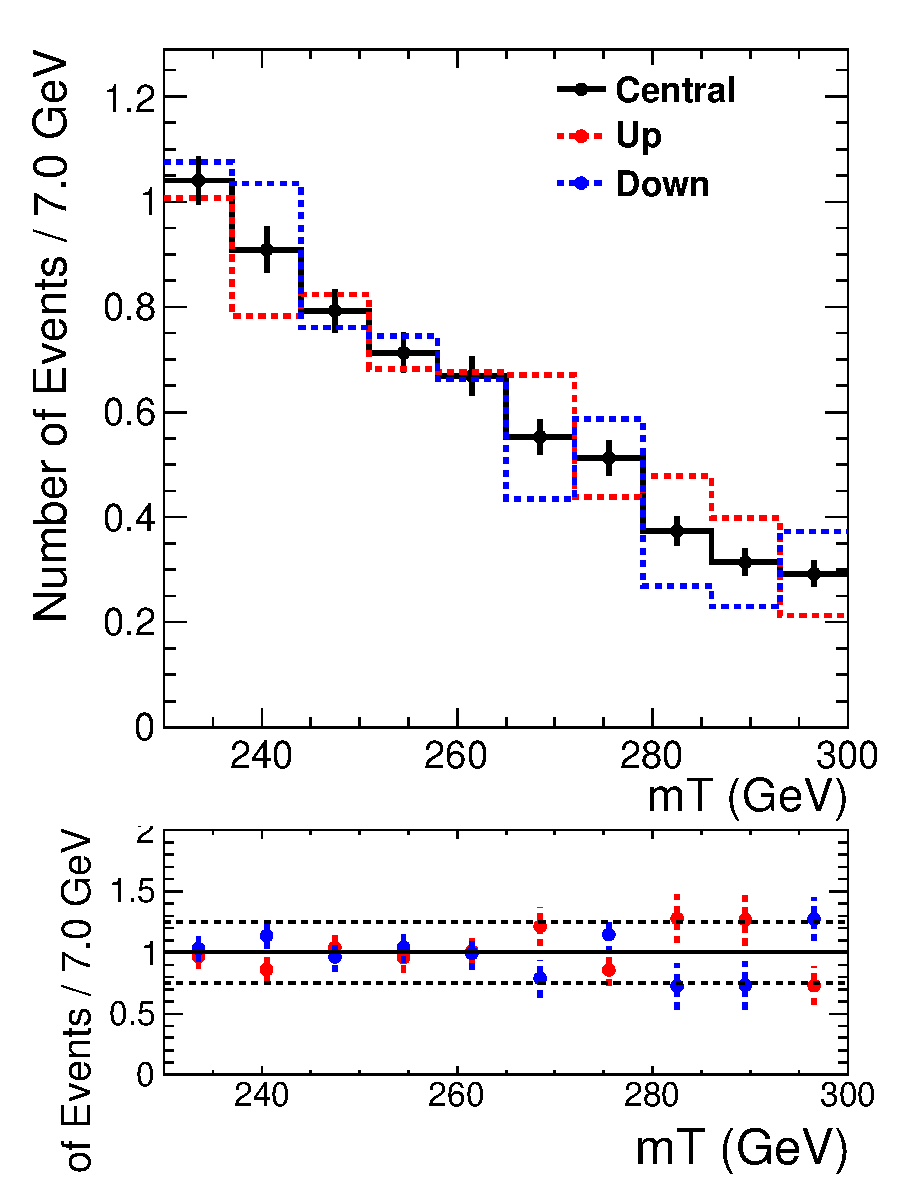
\includegraphics[width=0.49\textwidth]{figures/WZ_WZBounding_mT_mH250_ee_lin.pdf}}
\subfigure[]{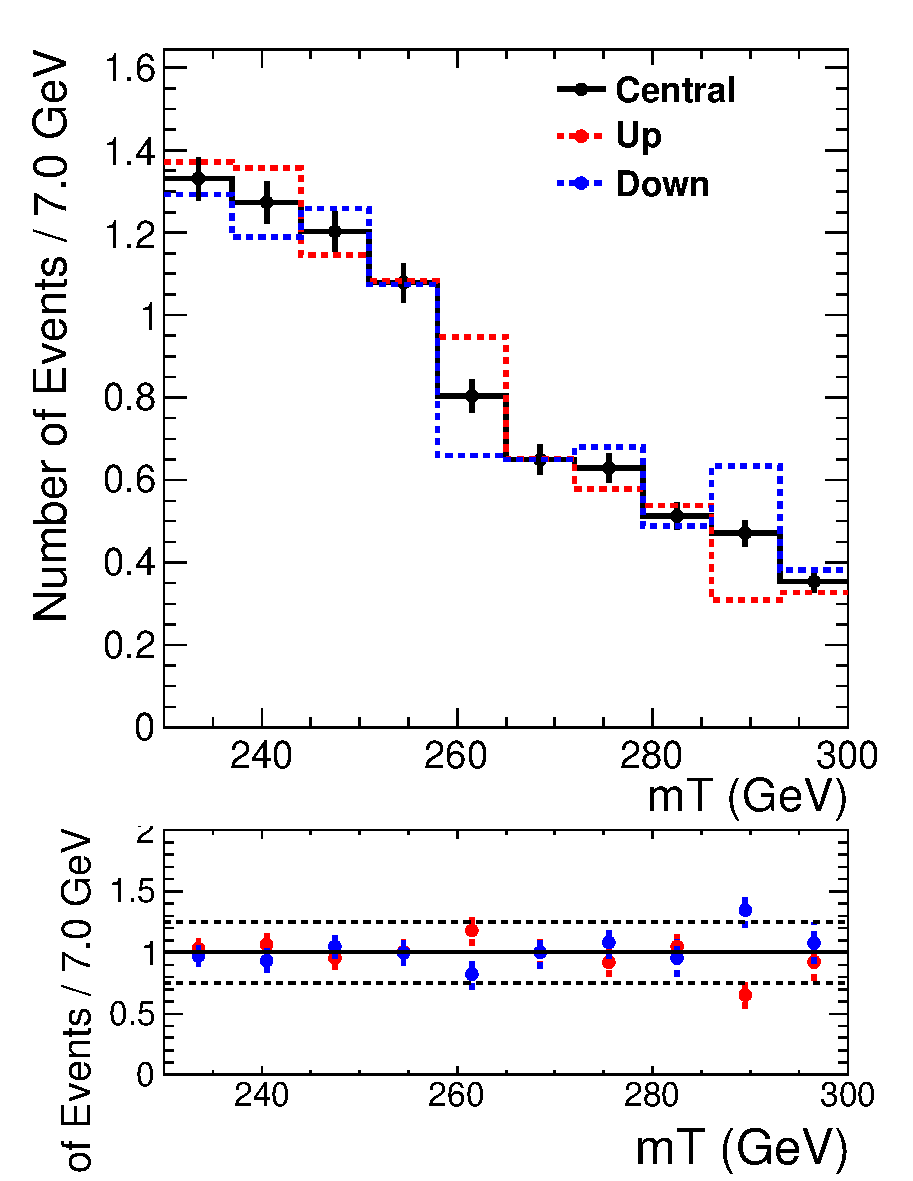
\includegraphics[width=0.49\textwidth]{figures/WZ_WZBounding_mT_mH250_mm_lin.pdf}}\\
\caption{$m_T$ distribution for $\WZ$ for the ee (left) and $\mu\mu$ (right) final states. 
The central shape is taken from Madgraph with $p_T$ spectrum reweighted to match 
the NLO calcuation. The up histogram is taken from Pythia with the down 
histogram taken as a variation mirroring the difference between up and central. 
}
\label{fig:wzsyst_hzz}
\end{center}
\end{figure}
%%%%%%%%%%%%%%%%%%%%%%%%
\subsection{Top and \WW\   Background}

For the Top and \WW{} background involving the $\mu^+\mu^-$, $e^+\mu^-$ and 
$e^+e^-$ that occur with equal rates ( after correcting the electron 
to muon efficiency ratio), we can estimate the shapes from data using 
the opposite flavor ($e^\pm\mu^\mp$ states. To ensure the kinematics 
in the opposite flavor states to be the same as in the same flavors, we 
need to apply the same selections in the signal region. The 
statistics is rather limited after the $\met$ preselections and 
b-tagging veto as shown in Fig.~\ref{fig:mtemdatamc}. 

However the top background $m_T$ distributions are not sensitive to the 
tagging of the b-quark or the dilepton flavors to the first approximation. 
Therefore, we can enrich top background statisitcs by defining a 
top enriched control region, where we relaxing the btag requirement 
in all the dilepton final states. Figure~\ref{fig:mtcompsigcontrl} 
compares the $m_T$ distributions between the same flavor signal region and 
the control region and found the two regions give consistent spectrum. 
Figure~\ref{fig:mtdatamcl} shows the comparison of the $m_T$ 
distributions between the signal MC region and the control region in both data and MC. 
Therefore we can use the shapes in the signal regional derived from MC 
as the central shape and place the shapes in the control region derived from Data as the 
alternative, as shown in Figure~\ref{fig:topsyst_hzz} for the $m_H=250\GeVcc$ selection. 

Seperating the top background, the \WW{} background shape variations can be assessed 
in the same way as in the $\hww$ analysis described in the previous section. 
Figure~\ref{fig:wwsyst_hzz}-\ref{fig:wwnlosyst_hzz} show the variations we consider 
for the $m_H=250\GeVcc$ selection. 

%%%%%%%%%%%%%%
\begin{figure}[!htbp]
\begin{center}
\subfigure[]{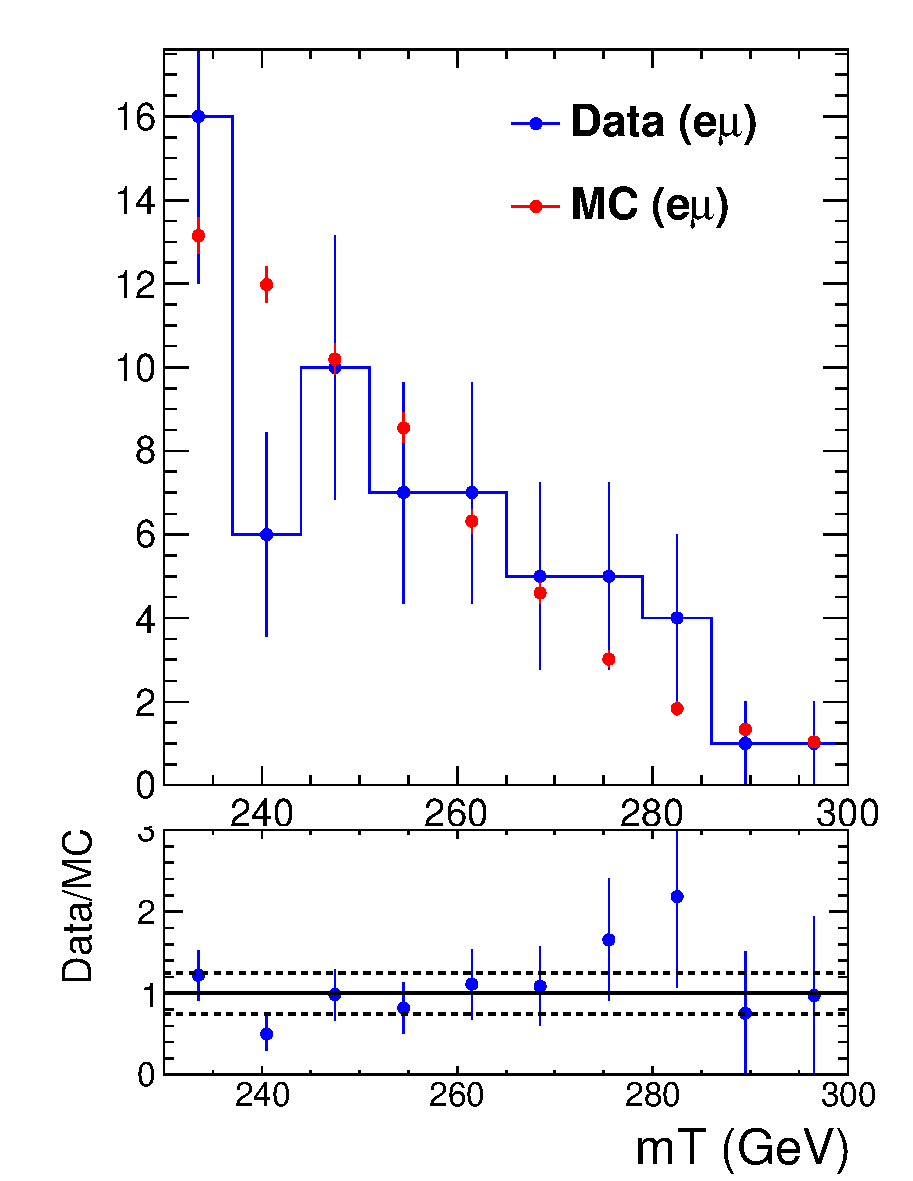
\includegraphics[width=0.49\textwidth]{figures/OF_mT_mH250_datamc_lin.pdf}}\\
\caption{Comparing the $m_T$ transverse mass distribution in the opposite flavor between data and MC.The data corresponds to 1.1/fb.}
\label{fig:mtemdatamc}
\end{center}
\end{figure}
%%%%%%%%%%%%%%

%%%%%%%%%%%%%%
\begin{figure}[!htbp]
\begin{center}
\begin{tabular}{cc}
\subfigure[]{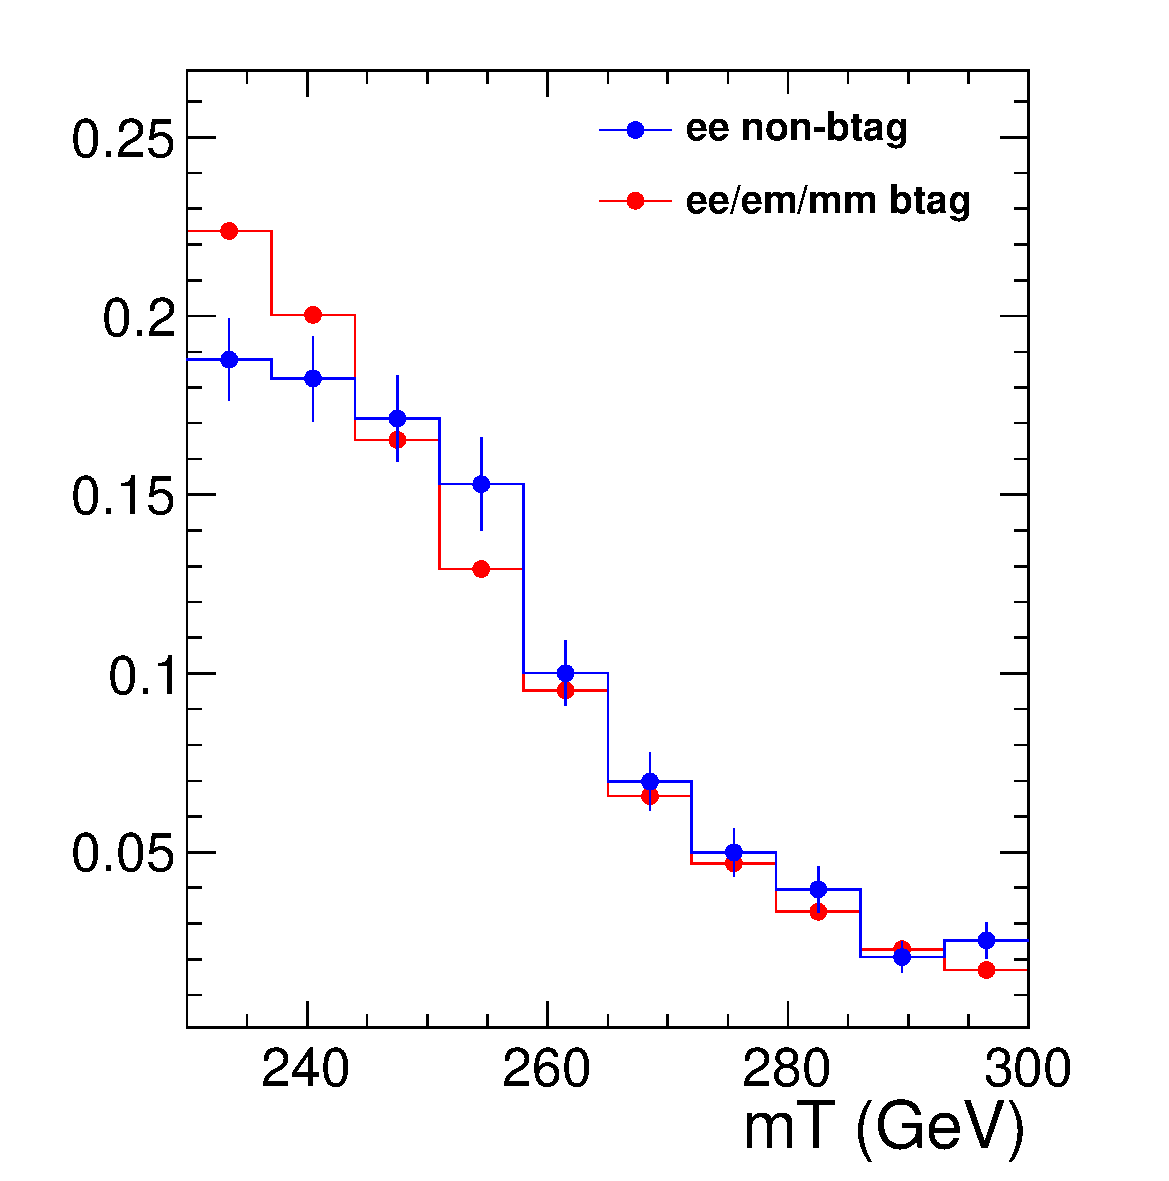
\includegraphics[width=0.49\textwidth]{figures/Top_mT_mH250_ee_lin.pdf}}
\subfigure[]{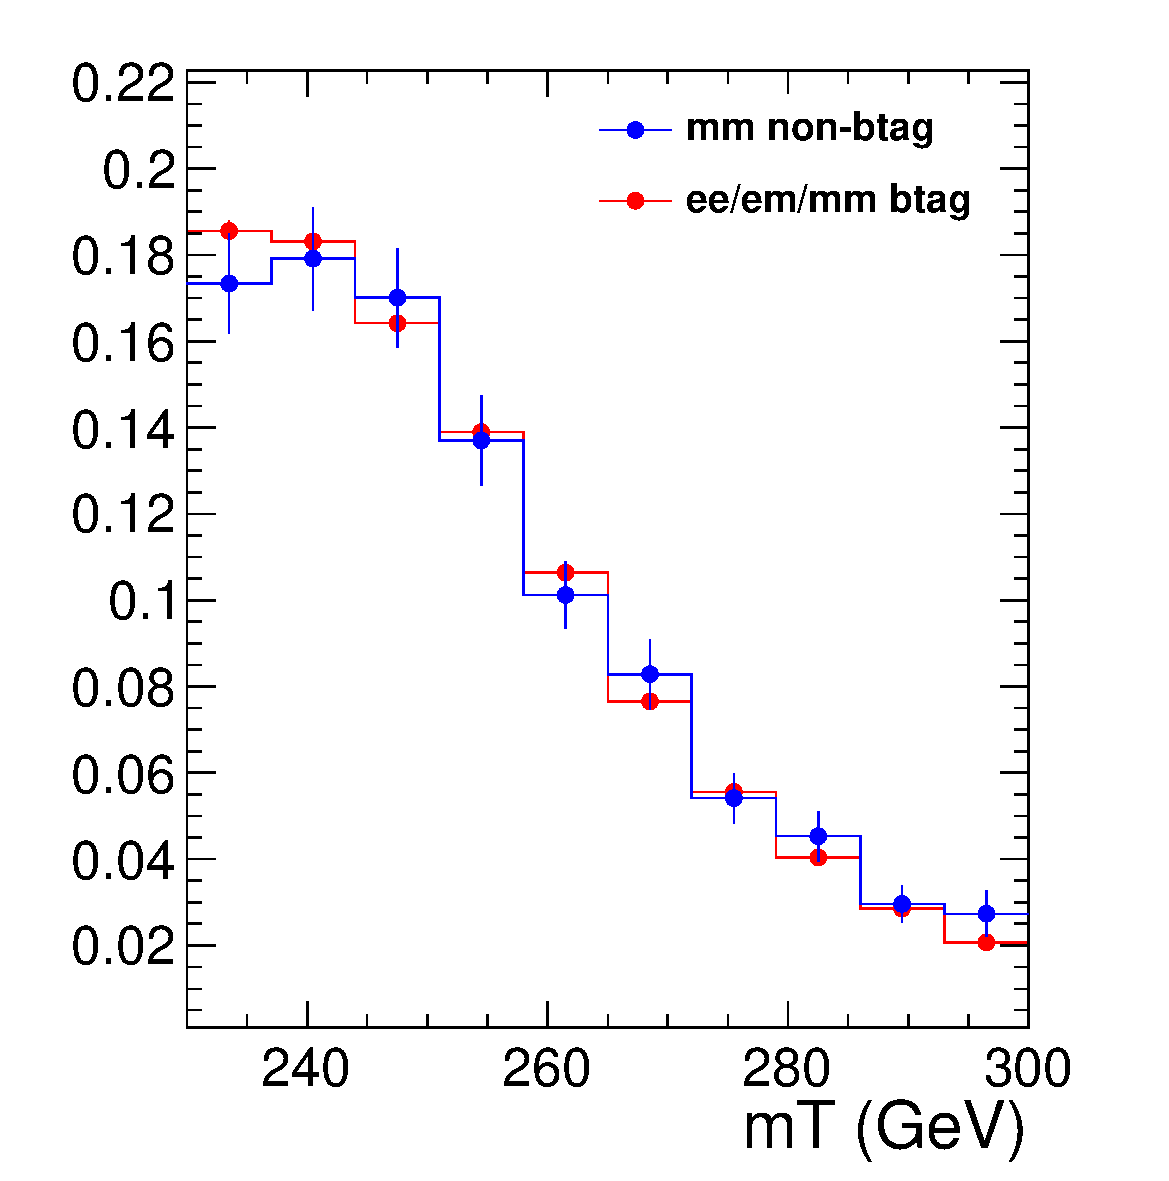
\includegraphics[width=0.49\textwidth]{figures/Top_mT_mH250_mm_lin.pdf}}\\
\end{tabular}
\caption{Comparing the mT distribution in the $H\to ZZ$ signal region and the top enriched control region in $ee/\mu\mu$ final states. This is evaluated with the $mH=250$ selections. }
\label{fig:mtcompsigcontrl}
\end{center}
\end{figure}
%%%%%%%%%%%%%%

%%%%%%%%%%%%%%
\begin{figure}[!htbp]
\begin{center}
\begin{tabular}{cc}
\subfigure[]{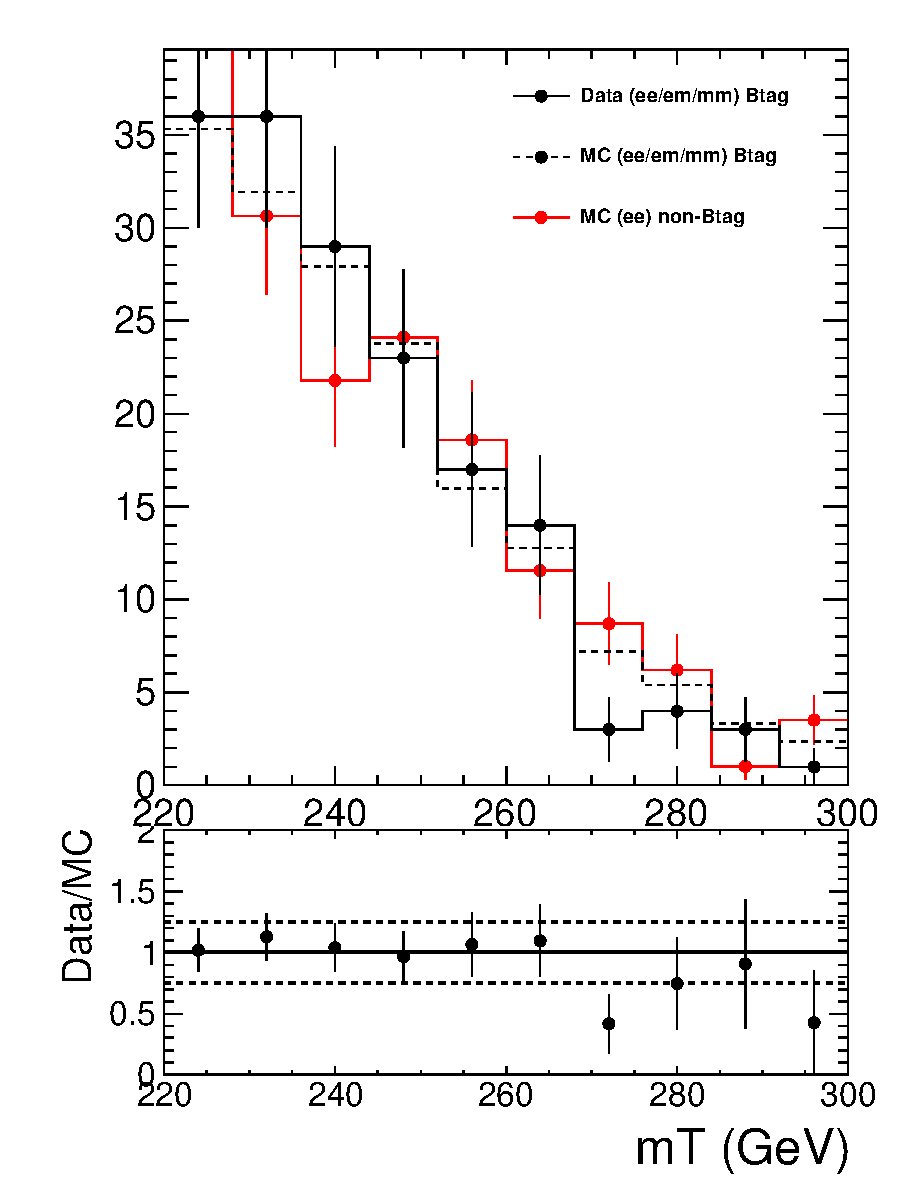
\includegraphics[width=0.49\textwidth]{figures/Top_mT_mH250_datamc_ee_lin.pdf}}
\subfigure[]{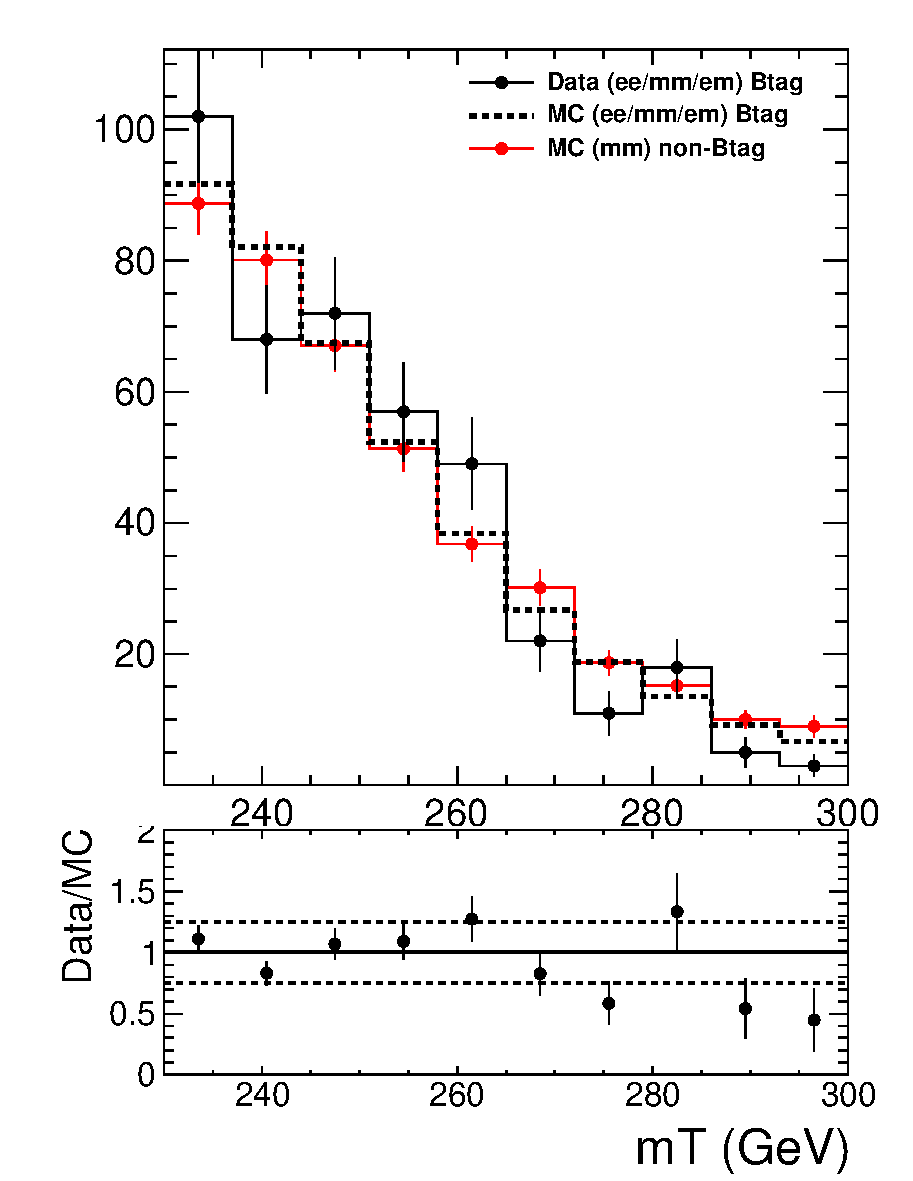
\includegraphics[width=0.49\textwidth]{figures/Top_mT_mH250_datamc_mm_lin.pdf}}\\
\end{tabular}
\caption{Comparing the mT distribution in the $H\to ZZ$ signal region in MC in $ee$ (left) and $\mu\mu$ (right) and the top enriched control region in all dilepton final states requiring btagging. This is evaluated with the $mH=250$ selections. }
\label{fig:mtdatamcl}
\end{center}
\end{figure}
%%%%%%%%%%%%%%



%%%%%%%%%%%%%%%%%%%%%%%%
\begin{figure}[!htbp]
\begin{center}
\subfigure[]{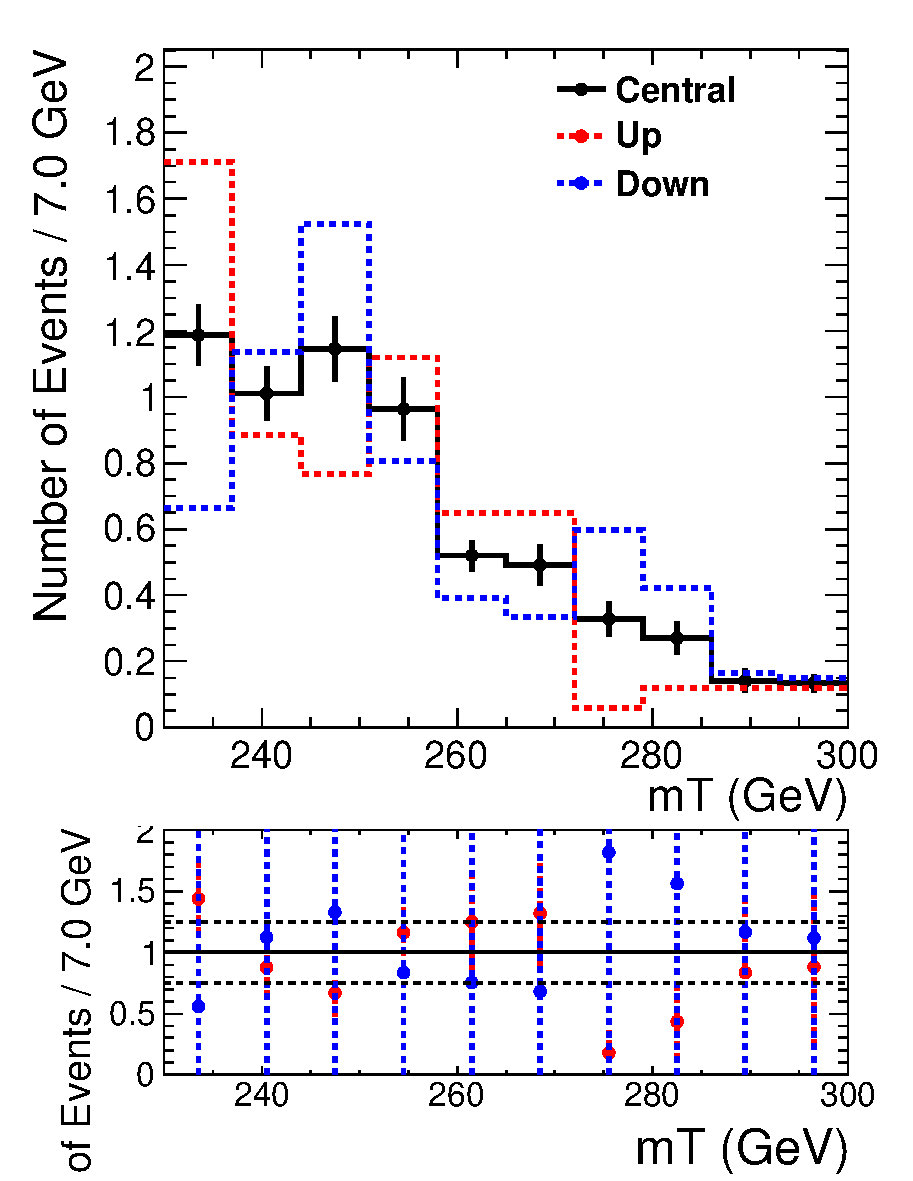
\includegraphics[width=0.49\textwidth]{figures/Top_TopBounding_mT_mH250_ee_lin.pdf}}
\subfigure[]{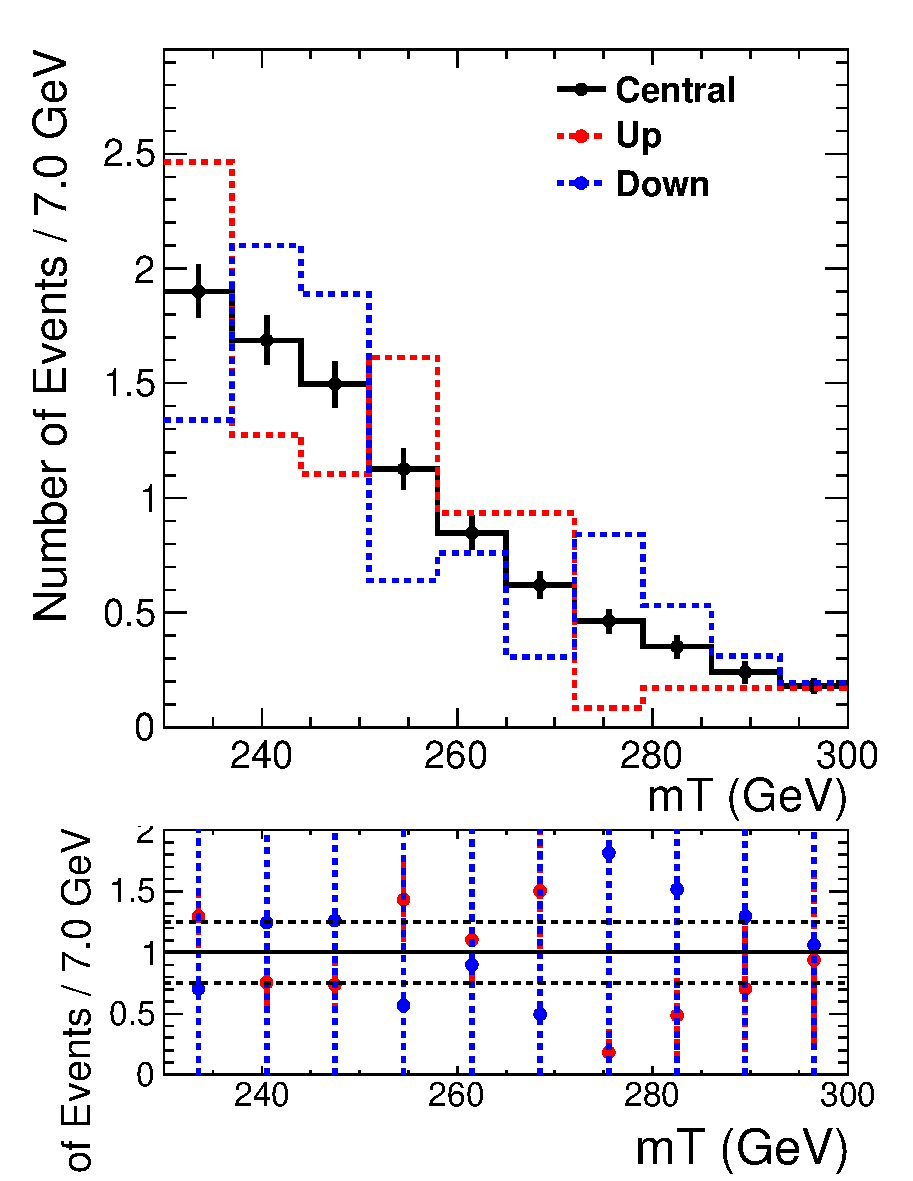
\includegraphics[width=0.49\textwidth]{figures/Top_TopBounding_mT_mH250_mm_lin.pdf}}\\
\caption{$m_T$ distribution for Top for the ee (left) and $\mu\mu$ (right) final states. 
The central shape is taken from MC in the signal region. The up histogram is taken from 
data in the control region, with the down 
histogram taken as a variation mirroring the difference between up and central. 
}
\label{fig:topsyst_hzz}
\end{center}
\end{figure}
%%%%%%%%%%%%%%%%%%%%%%%%

%%%%%%%%%%%%%%%%%%%%%%%%
\begin{figure}[!htbp]
\begin{center}
\subfigure[]{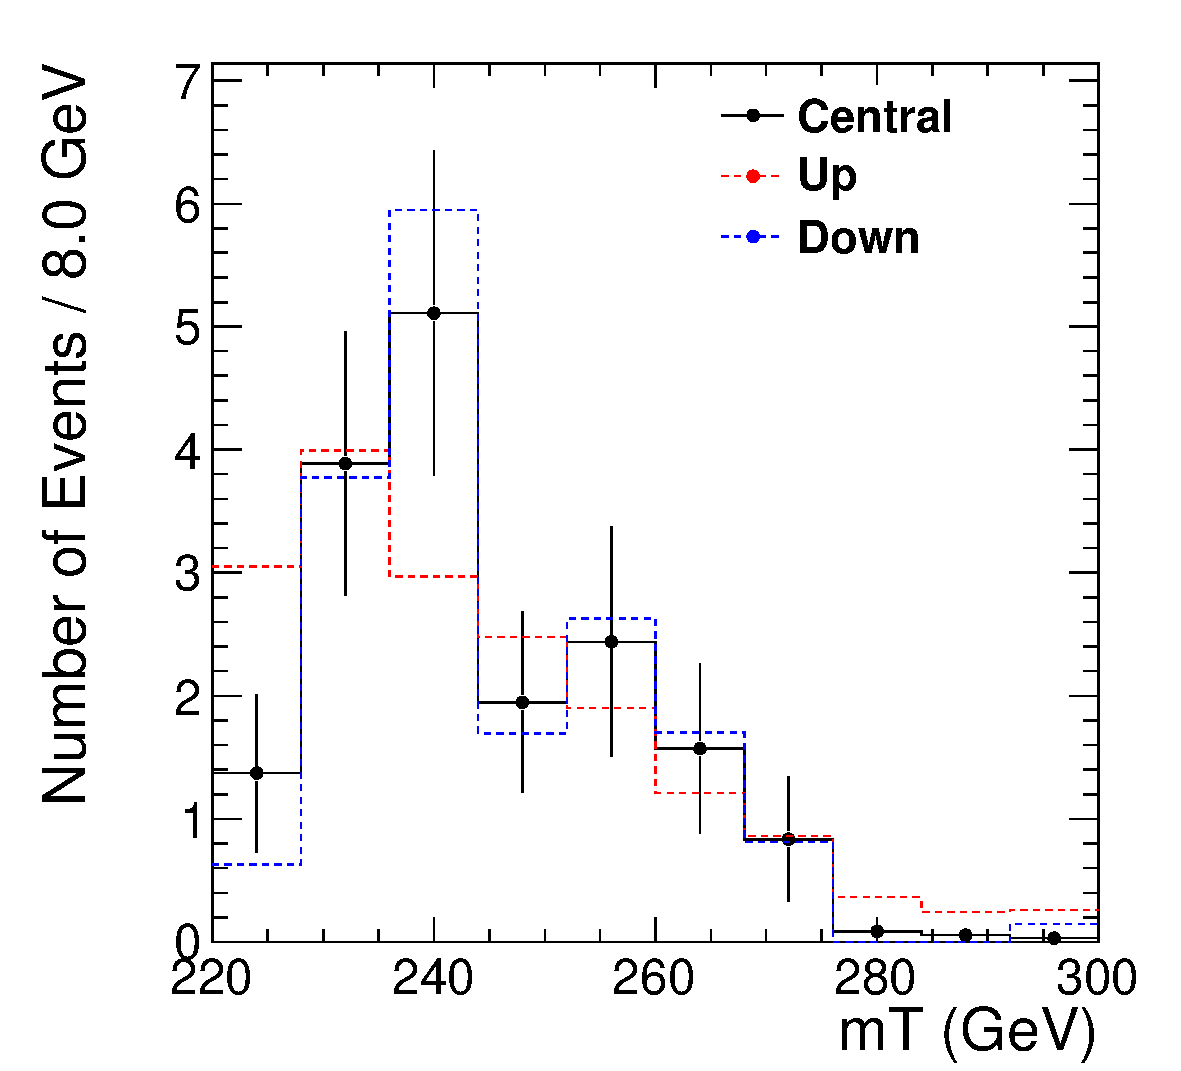
\includegraphics[width=0.49\textwidth]{figures/WW_WWBounding_mT_mH250_ee_lin.pdf}}
\subfigure[]{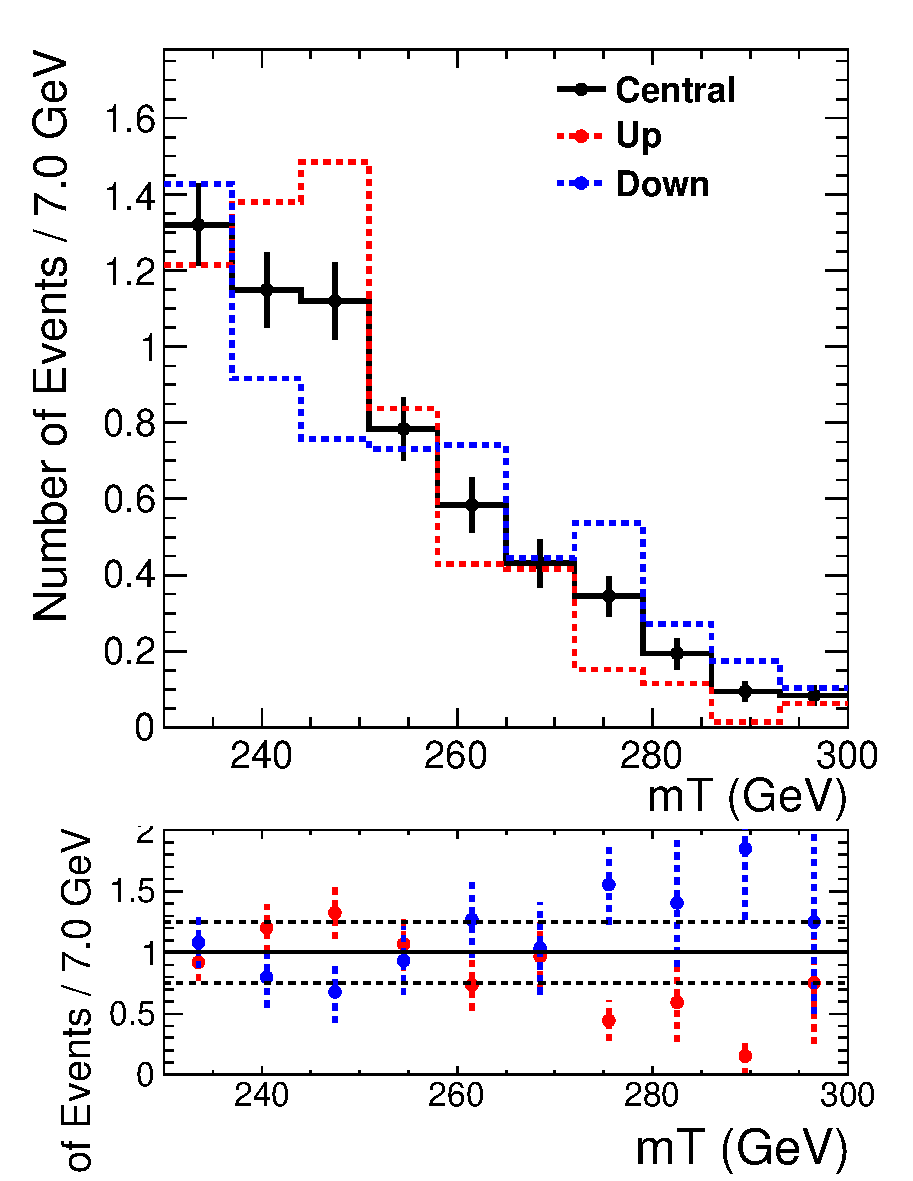
\includegraphics[width=0.49\textwidth]{figures/WW_WWBounding_mT_mH250_mm_lin.pdf}}\\
\caption{$m_T$ distribution for WW for the ee (left) and $\mu\mu$ (right) final states. 
The central shape is taken from Pythia MC. The up histogram is taken from 
MC@NLO, with the down histogram taken as a variation mirroring the difference between up and central. 
}
\label{fig:wwsyst_hzz}
\end{center}
\end{figure}
%%%%%%%%%%%%%%%%%%%%%%%%
%%%%%%%%%%%%%%%%%%%%%%%%
\begin{figure}[!htbp]
\begin{center}
\subfigure[]{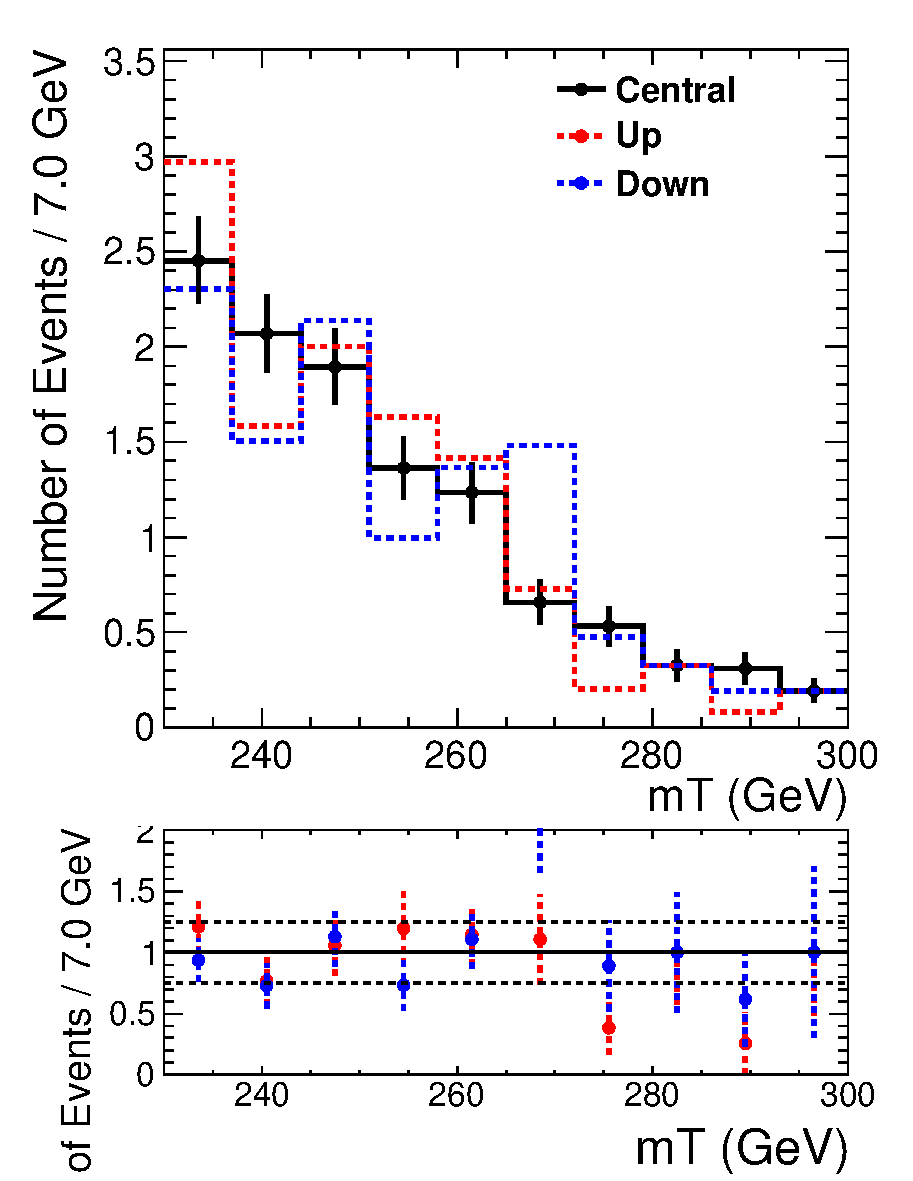
\includegraphics[width=0.49\textwidth]{figures/WW_WWNLOBounding_mT_mH250_ee_lin.pdf}}
\subfigure[]{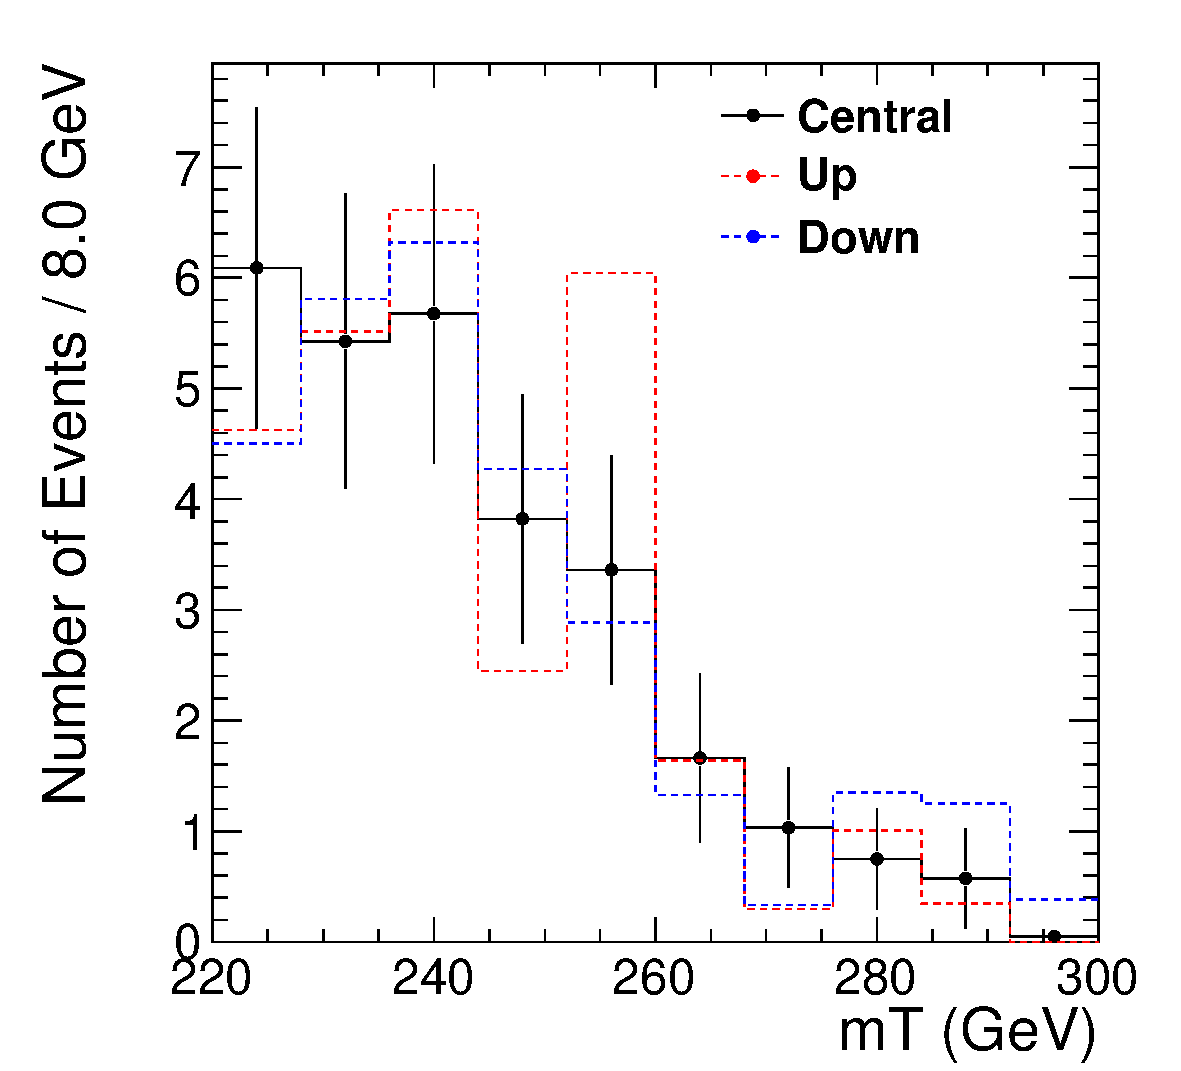
\includegraphics[width=0.49\textwidth]{figures/WW_WWNLOBounding_mT_mH250_mm_lin.pdf}}\\
\caption{$m_T$ distribution for WW for the ee (left) and $\mu\mu$ (right) final states. 
The central shape is taken from Pythia MC. The up/down histogram accounts for the QCD scaling up effect
derived from MC@NLO and scaled to the central shape. 
}
\label{fig:wwnlosyst_hzz}	
\end{center}
\end{figure}
%%%%%%%%%%%%%%%%%%%%%%%%

\subsection{\dyll\  Background}

The \dyll\  background shape can be estimated from data in the $m_T$ and BDT based 
shape analysis. This is because in both method we only use the dilepton momentum 
instead of the individual lepton information as in the matrix element method. 
The intrinsic difference between the photon jet and Z jets events is partially
accounted for in the overal normalization uncertainty. 
The lack of statistics in the \dyll\  background makes the comparison of the 
data-driven shape and the MC shape in the signal region difficult. 
If sufficient MC statistics is available, we can use the shape in the signal region in MC as 
the alternative shape to interpreted as the one sigma variation. 




